\documentclass[12pt,a4paper]{report}

\usepackage[spanish,es-tabla]{babel}
\usepackage[utf8]{inputenc}
\usepackage[T1]{fontenc}
% Helvetica como sustituto métrico de Arial (Arial real requiere XeLaTeX/Overleaf).
\usepackage{helvet}
\renewcommand{\familydefault}{\sfdefault}

% Justificación a ambos lados (comportamiento por defecto de report; se deja explícito).
\usepackage{ragged2e}

\usepackage[
  top=3cm, bottom=3cm, left=3cm, right=3cm,
  headheight=15pt, headsep=10pt
]{geometry}
\usepackage{setspace}
\setstretch{1.15}              % Interlineado 1,15 (requisito de formato)
\setlength{\parindent}{1.25cm}
\setlength{\parskip}{0.5em}

\usepackage[table]{xcolor}
% tikz debe cargarse antes de tikz-paleta porque este usa \tikzset.
\usepackage{tikz}
\usetikzlibrary{positioning, arrows.meta, shapes.geometric}
% Paleta alineada con frontend/css/dr-agramonte.css
\definecolor{teal}{RGB}{15,118,110}
\definecolor{tealdark}{RGB}{19,78,72}
\definecolor{teallight}{RGB}{20,184,166}
\definecolor{tealpale}{RGB}{240,253,250}
\definecolor{silver}{RGB}{212,212,216}
\definecolor{offwhite}{RGB}{249,250,251}
\definecolor{graytext}{RGB}{107,114,128}
\definecolor{graydark}{RGB}{31,41,55}
\definecolor{carddark}{RGB}{30,41,59}
\definecolor{bgdark}{RGB}{15,23,42}
\definecolor{rowgray}{RGB}{243,244,246}
\definecolor{bordergray}{RGB}{229,231,235}
\definecolor{codebg}{RGB}{30,41,59}
\definecolor{codefg}{RGB}{226,232,240}

% Alias compatibles con el estilo anterior
\colorlet{darkblue}{tealdark}
\colorlet{medblue}{teal}
\colorlet{lightblue}{tealpale}

\tikzset{
  block/.style={
    draw=teal, rounded corners=10pt, line width=0.9pt,
    fill=tealpale, text=graydark, font=\small\sffamily,
    minimum height=1.1cm, align=center, inner sep=6pt
  },
  blockdark/.style={
    block, fill=carddark, text=white, draw=teallight
  },
  blockaccent/.style={
    block, fill=teal!85!black, text=white, draw=tealdark
  },
  arrow/.style={->, >=Stealth, line width=0.9pt, teal},
  entity/.style={
    draw=teal, fill=tealpale, rounded corners=6pt,
    font=\small\sffamily, align=center, inner sep=5pt
  },
  rel/.style={->, >=Stealth, teal, line width=0.7pt}
}


\usepackage{amssymb}
\usepackage{pifont}
\DeclareUnicodeCharacter{2713}{\checkmark}

\usepackage{fancyhdr}
\pagestyle{fancy}
\fancyhf{}
\fancyhead[L]{\small\color{tealdark}Mar Agramonte --- Dr. Agramonte}
\fancyhead[R]{\small\thepage}
\renewcommand{\headrulewidth}{0.4pt}

\usepackage{titlesec}
\titleformat{\chapter}[display]
  {\normalfont\Large\bfseries\color{tealdark}}
  {Capítulo \thechapter:}{16pt}{\Large}
\titleformat{\section}{\normalfont\large\bfseries\color{tealdark}}{\thesection}{1em}{}
\titleformat{\subsection}{\normalfont\normalsize\bfseries\color{teal}}{\thesubsection}{1em}{}

\usepackage{tocloft}
\renewcommand{\cftchapfont}{\bfseries\color{tealdark}}
\renewcommand{\cftchappagefont}{\bfseries\color{tealdark}}

\usepackage{booktabs, array, longtable, float, caption}
% Figuras, tablas y leyendas a tamaño 10 (requisito de formato).
\captionsetup{font=footnotesize,labelfont={bf,color=tealdark}}

\usepackage{listings}
\lstdefinestyle{mycode}{
  backgroundcolor=\color{codebg},
  basicstyle=\ttfamily\footnotesize\color{codefg},
  breaklines=true, numbers=left, numbersep=8pt,
  frame=single, framerule=0pt, xleftmargin=14pt,
}
\lstset{style=mycode}

\usepackage{graphicx}
% tikz y sus librerías ya se cargan al inicio (antes de tikz-paleta).

\usepackage{hyperref}
\hypersetup{
  colorlinks=true, linkcolor=tealdark, urlcolor=teal, citecolor=tealdark,
  pdftitle={Dr. Agramonte - Gestión de Citas Médicas},
  pdfauthor={Mar Agramonte},
}

\newcommand{\hrow}{\rowcolor{tealpale}}
\newcommand{\grayrow}{\rowcolor{rowgray}}

\begin{document}

% --- Portada (sin número de página) ---
\begin{titlepage}
  \pagestyle{empty}
  \centering
  \vspace*{1.5cm}
  {\Large\bfseries\color{tealdark} MEMORIA TÉCNICA DEL PROYECTO\\[0.8em]}
  \vspace{0.8cm}
  {\Huge\bfseries\color{teal} DR. AGRAMONTE\\[0.4em]}
  {\Large\bfseries\color{teallight} Plataforma web de gestión de citas médicas\\[1.5em]}
  \begin{tikzpicture}
    \fill[tealpale, rounded corners=12pt] (0,0) rectangle (12,0.35);
    \fill[teal] (0,0) rectangle (4,0.35);
  \end{tikzpicture}
  \vfill
  \begin{tabular}{rl}
    \textbf{Autora:} & Mar Agramonte Campos \\
    \textbf{En línea:} & \url{https://www.dragramonte.com} \\
  \end{tabular}
\end{titlepage}

\clearpage
\pagestyle{fancy}
\setcounter{page}{1}

% ============================================================================
% RESUMEN (se redacta al final; recoge ideas clave y conclusiones)
% ============================================================================
\chapter*{Resumen}
\addcontentsline{toc}{chapter}{Resumen}

\textbf{Dr. Agramonte} es una aplicación web para que pacientes reserven, consulten y cancelen citas médicas sin depender del teléfono del profesional. El sistema integra un frontend estático (HTML, CSS y JavaScript), una API REST con \textbf{Spring Boot 3.5.3}, base de datos \textbf{PostgreSQL}, autenticación \textbf{JWT}, control de concurrencia con \textbf{bloqueo pesimista}, notificaciones por dos canales independientes —\textbf{Twilio} (SMS/WhatsApp) y un \textbf{bot de Telegram}— y despliegue reproducible con \textbf{Docker Compose}. La aplicación está además \textbf{desplegada en la nube y es accesible públicamente con HTTPS} en \url{https://www.dragramonte.com}.

El proyecto nace de una observación directa del sector sanitario: buena parte de las llamadas que recibe un médico fuera de su horario no son urgencias clínicas, sino gestión de agenda. Digitalizar esa parte administrativa devuelve tiempo al profesional sin sustituir el trato humano donde de verdad hace falta. Sobre esa idea se construye una herramienta pensada para consultas pequeñas y médicos autónomos, que mantienen la titularidad de sus datos en lugar de depender de plataformas de terceros.

La interfaz replica la identidad visual del consultorio: paleta \textbf{teal} (\#0F766E, \#14B8A6), tipografías DM Sans / DM Serif Display, modo claro/oscuro y diseño responsive. La reserva se organiza en pasos (centro, calendario, hora, datos y confirmación) y puede iniciarse desde \texttt{servicios.html} con el tipo de consulta preseleccionado. Un \textbf{cuadro de mando} restringido por rol convierte los datos operativos en información de gestión (carga por médico, demanda por especialidad, tasa de cancelación) y la interfaz sigue las pautas de accesibilidad \textbf{WCAG 2.1 AA}.

La calidad se respalda con una batería de \textbf{pruebas automatizadas} (unitarias, de seguridad y de integración con Testcontainers) y con análisis de vulnerabilidades \textbf{OWASP dependency-check}. La principal conclusión es que la coherencia entre memoria, código y demostración es tan determinante como la propia funcionalidad: este documento describe la versión \emph{real} del sistema —la que está desplegada y en funcionamiento—, distinguiendo en todo momento lo entregado de lo planificado como evolución.

\vspace{0.5em}
\noindent\textbf{Palabras clave:} citas médicas, aplicación web, Spring Boot, API REST, PostgreSQL, JWT, concurrencia, Twilio, Telegram, Docker, despliegue en la nube, HTTPS, PWA, accesibilidad.

% ============================================================================
\chapter*{Abstract}
\addcontentsline{toc}{chapter}{Abstract}
% ============================================================================

\textbf{Dr. Agramonte} is a web application that lets patients book, review and cancel medical appointments without depending on the practitioner's phone line. The system integrates a static frontend (HTML, CSS and JavaScript), a REST API built with \textbf{Spring Boot 3.5.3}, a \textbf{PostgreSQL} database, \textbf{JWT} authentication, concurrency control through \textbf{pessimistic locking}, notifications over two independent channels —\textbf{Twilio} (SMS/WhatsApp) and a \textbf{Telegram bot}— and reproducible deployment with \textbf{Docker Compose}. The application is also \textbf{deployed to the cloud and publicly accessible over HTTPS} at \url{https://www.dragramonte.com}.

The project stems from direct observation of the healthcare sector: many of the calls a doctor receives outside working hours are not clinical emergencies but scheduling tasks. Digitising that administrative layer gives time back to the professional without replacing human contact where it is truly needed. On this premise, the tool is designed for small practices and self-employed doctors, who retain ownership of their data instead of relying on third-party platforms.

The interface mirrors the practice's visual identity: a \textbf{teal} palette (\#0F766E, \#14B8A6), DM Sans / DM Serif Display typefaces, light/dark mode and responsive design. Booking is organised in steps (centre, calendar, time, details and confirmation) and can be started from \texttt{servicios.html} with the appointment type preselected. A role-restricted \textbf{management dashboard} turns operational data into business insight (workload per doctor, demand per specialty, cancellation rate), and the interface follows \textbf{WCAG 2.1 AA} accessibility guidelines.

Quality is backed by a suite of \textbf{automated tests} (unit, security and Testcontainers-based integration) and \textbf{OWASP dependency-check} vulnerability analysis. The main conclusion is that consistency between report, code and demonstration is as decisive as functionality itself: this document describes the \emph{real} state of the system —the one deployed and running—, consistently distinguishing what has been delivered from what is planned as future work.

\vspace{0.5em}
\noindent\textbf{Keywords:} medical appointments, web application, Spring Boot, REST API, PostgreSQL, JWT, concurrency, Twilio, Docker, cloud deployment, HTTPS, PWA, accessibility.

\clearpage
\tableofcontents
\newpage

% ============================================================================
\chapter{Justificación y contexto}
% ============================================================================

\section{De dónde viene este proyecto}

Me he criado rodeada de sanidad. La mayoría de mis familiares y amigos trabajan en el sector, así que lo que sé de esta profesión no viene de un libro: viene de haberla visto de cerca durante años. Y lo que he visto se repite con una regularidad que asusta: un médico no desconecta cuando cierra la consulta. El teléfono sigue sonando. En Navidad, en verano, en mitad de una cena, incluso en mitad de un viaje. Siempre hay alguien que llama, ya sea para confirmar una cita, preguntar por una receta o pedir un consejo que, sinceramente, podría esperar.

La mayoría de esas llamadas no son urgencias. Son gestiones que, con la herramienta adecuada, el paciente podría resolver por su cuenta. Lo que muchas veces se pasa por alto es que ese médico también tiene familia, también necesita estar en una cena sin el teléfono encima y también tiene derecho a un domingo sin interrupciones. La tecnología no lo soluciona todo, pero sí puede encargarse de la parte administrativa que hoy recae directamente sobre el profesional. De ahí nace este proyecto: no es una idea inventada, es algo que observé durante años. Si el paciente puede gestionar sus citas solo, el médico recupera tiempo. Es así de simple.

\section{La carga administrativa invisible}

El problema no es solo cuántas llamadas entran, es quién acaba cogiéndolas. En muchas consultas pequeñas, o en centros que van desbordados, no hay personal de administración, así que el médico termina haciendo también ese trabajo. Cada vez que descuelga el teléfono para confirmar una cita o resolver un trámite, deja a medias lo que estaba haciendo con el paciente que tiene delante.

Este proyecto no quiere sustituir el trato humano ni apartar al profesional del teléfono. Hay momentos en los que quien llama está asustado, confuso o simplemente necesita que alguien lo escuche, y para eso no vale una aplicación. Lo que busco es que el médico no tenga que coger el teléfono cada vez que alguien llama para confirmar que su cita del jueves sigue siendo a las cinco, ni cada vez que un paciente aprovecha que tiene su número para preguntar una duda que podría esperar a la próxima consulta. Eso sí lo puede hacer un sistema, y liberar ese tiempo es, en el fondo, el objetivo de toda la plataforma.

\section{El coste oculto para el profesional}

Hay algo que casi nunca se dice en voz alta. Cuando el médico sale de la consulta por la tarde, no deja de ser médico: sigue pendiente. Si un paciente le llama a las diez de la noche porque le duele algo, coge el teléfono. Si alguien le escribe un domingo por la mañana, contesta. Y todas esas horas en las que está trabajando, aunque nadie lo llame trabajo, no las cobra: están fuera de su jornada, fuera de su sueldo y dentro de su vida.

Y hay algo más que tampoco suele mirarse: nadie pregunta si el médico está bien, si ha dormido, si ha comido, si lleva semanas arrastrando un cansancio que no se permite parar. Como su oficio es cuidar, damos por hecho que ya se cuida solo, y muchas veces no es así. Lo he visto en gente de mi familia y en amigos del sector: pasan el día entero escuchando lo que le duele a todo el mundo y llegan a casa sin margen para contar lo suyo. Por eso entiendo esta aplicación no solo como un gestor de citas, sino como una pequeña forma de devolver un respiro a alguien que llevaba mucho tiempo sin pedirlo.

\section{El hueco que existe en el mercado}

En España, si trabajas en un hospital grande tienes sistemas de cita online; si formas parte de una clínica privada importante, tienes acceso a plataformas como Doctoralia o Top Doctors. Pero si eres un médico independiente o ejerces en una consulta pequeña, lo más probable es que sigas gestionando las citas por teléfono y agenda de papel. Las soluciones existentes presentan carencias para ese perfil:

\begin{itemize}
  \item \textbf{Comisiones y suscripciones} pensadas para grandes volúmenes, que no encajan con quien atiende a 40--50 pacientes a la semana.
  \item \textbf{Dependencia de terceros:} el médico deja de ser dueño de sus propios datos, que pasan a alojarse en servidores ajenos.
  \item \textbf{Personalización limitada:} no se adaptan con facilidad a una especialidad concreta ni al modo de trabajar de una consulta pequeña.
\end{itemize}

Existe un espacio entre ambas opciones donde caben muchos profesionales que necesitan una herramienta especializada, accesible y bajo su control. \textbf{Dr. Agramonte se diseña pensando precisamente en ese espacio.}

\section{El sector: construir software para una consulta médica}

El ámbito del proyecto es el sanitario privado y, dentro de él, un problema muy concreto: la gestión de agenda, la relación paciente--médico y la comunicación entre ambos.

Construir software para una consulta médica exige un perfil mixto: por un lado, trabajo de oficina propio del desarrollo de software (análisis, programación, pruebas, documentación); por otro, la necesidad de entender la realidad de un entorno clínico, donde los datos que se manejan son sensibles, los usuarios tienen edades y niveles digitales muy distintos, y un error no es un simple \emph{bug}, sino una persona afectada. Comprender ese sector —sus tiempos, sus prioridades y sus límites legales— es tan parte del trabajo como escribir el código, y de hecho condiciona casi todas las decisiones técnicas que aparecen más adelante.

\section{Tipos de solución y dónde encaja el proyecto}

Desde el punto de vista del desarrollo, una herramienta de gestión de citas puede abordarse de tres formas, cada una con sus compromisos:

\begin{itemize}
  \item \textbf{SaaS} (software como servicio): el proveedor aloja la aplicación y el cliente paga una suscripción (Doctoralia, Top Doctors). Cómodo y siempre actualizado, pero con costes recurrentes, comisiones y los datos en manos de un tercero.
  \item \textbf{A medida} (\emph{open source} / propietario): la aplicación se desarrolla y se despliega en la infraestructura del propio profesional. Da control total, sin comisiones y permite personalizar, a cambio de requerir conocimiento técnico para mantenerla.
  \item \textbf{Herramientas genéricas} (agendas o CRM no sanitarios): baratas, pero ajenas a las particularidades de la sanidad (historial clínico, normativa de conservación, roles).
\end{itemize}

\textbf{Dr. Agramonte} se sitúa en el modelo \emph{a medida}: una solución propia, sin comisiones, con los datos bajo control del consultorio y pensada para ser desplegable y mantenible por un perfil técnico.

\section{Viabilidad económica (estimación)}

Como desarrolladora, una decisión técnica no se sostiene solo por ser elegante: tiene que tener sentido también en coste. Por eso conviene una estimación, con cifras aproximadas y a modo ilustrativo, de lo que aporta la herramienta frente a su coste.

\textbf{Ahorro.} Si la reserva, confirmación y cancelación autónomas evitan en torno a \textbf{4 horas semanales} de gestión telefónica, y se valora la hora de consulta privada en unos 50\,€, el ahorro ronda los 200\,€ semanales, del orden de \textbf{10.000\,€ al año} en tiempo recuperado por el profesional.

\textbf{Coste.} El desarrollo es un coste \emph{único} ya asumido, y la operación es deliberadamente barata gracias a las decisiones de arquitectura: un frontend estático sin dependencias, un único backend Java y una base de datos relacional caben de sobra en una VPS modesta (del orden de 10\,€/mes). No hay comisiones por cita ni cuotas de plataforma de terceros.

\textbf{Conclusión.} Con estas cifras —que habría que afinar en un caso real— la inversión se amortiza en pocos meses. Más allá del número, la idea de fondo es que las decisiones de desarrollo (sin frameworks innecesarios, contenedores ligeros, una sola base de datos relacional) no solo simplifican el código: también hacen el sistema \textbf{sostenible} para una consulta pequeña.

Conviene situar el proyecto frente a las alternativas reales. Las grandes plataformas del sector privado (Doctoralia, Top Doctors) están pensadas para clínicas y hospitales con volúmenes altos: aportan visibilidad y un directorio de pacientes, pero a cambio el profesional depende de un intermediario, asume sus condiciones económicas y deja de ser dueño de sus propios datos. En el otro extremo, las herramientas genéricas de gestión (agendas o CRM no sanitarios) son más baratas, pero no entienden las particularidades de la sanidad: no contemplan historial clínico, no se ajustan a la normativa de conservación de datos de salud ni manejan roles propios de la práctica médica. Dr.\ Agramonte no compite con ninguno de los dos en su terreno; ocupa el hueco intermedio, ofreciendo a una consulta pequeña una solución propia, simple y conforme a la normativa, sin comisiones por cita ni dependencia de un tercero.

\section{Por qué y para qué}

\textbf{Por qué:} las consultas pequeñas y los médicos autónomos carecen de una herramienta de reserva propia, simple y bajo su control. \textbf{Para qué:} ofrecer un canal de autoservicio 24/7 que descargue al profesional de la gestión telefónica y mejore la experiencia del paciente, manteniendo la titularidad de los datos en manos del propio consultorio.

\section{Marco legal aplicable}

Cualquier aplicación que gestione datos de salud en Europa está sujeta a un marco legal exigente, precisamente porque se trata de información sensible:

\begin{itemize}
  \item \textbf{RGPD} (Reglamento (UE) 2016/679): los datos de salud son una categoría especial de datos, con un nivel de protección reforzado.
  \item \textbf{LOPDGDD} (Ley Orgánica 3/2018): la adaptación española del RGPD.
  \item \textbf{Ley 41/2002}, básica reguladora de la autonomía del paciente, que regula la documentación clínica y sus plazos de conservación.
\end{itemize}

Esto significa que no basta con que la aplicación funcione: tiene que funcionar de forma segura y conforme a la ley. La plataforma incorpora política de privacidad, consentimiento explícito en la reserva y minimización de datos (solo se piden los necesarios para gestionar la cita). Los datos son la intimidad de alguien que ha confiado en el sistema, y tratarlos con cuidado no es un extra: es la base.

% ============================================================================
\chapter{Objetivos}
% ============================================================================

Los objetivos se formularon con un criterio que ha guiado todo el proyecto: que cada meta fuera \textbf{concreta, verificable y realmente alcanzable} con los recursos disponibles. No se persigue prometer un producto enorme a medias, sino entregar un sistema más pequeño pero completo, coherente y demostrable.

\section{Objetivo general}

Desarrollar una aplicación web de gestión de citas médicas que permita al paciente reservar y cancelar de forma autónoma, reduciendo la dependencia del teléfono y devolviendo al profesional el control de su tiempo, sobre un backend seguro y un despliegue reproducible.

\section{Objetivos específicos}

Cada objetivo específico se corresponde con código real del repositorio y, cuando aplica, con una prueba que lo respalda. Esa trazabilidad entre objetivo, implementación y prueba es deliberada: evita el riesgo de prometer en la memoria lo que no existe en el sistema.

\begin{enumerate}
  \item Modelar y persistir usuarios, médicos, horarios y citas en \textbf{PostgreSQL} con migraciones \textbf{Flyway} y perfiles \texttt{postgres}/\texttt{mysql}.
  \item Implementar API REST con \textbf{Spring Boot}, autenticación \textbf{JWT} y roles \texttt{PACIENTE}, \texttt{MEDICO} y \texttt{ADMIN} en \texttt{SecurityConfig}.
  \item Garantizar integridad de reservas con \texttt{SELECT FOR UPDATE} sobre horarios disponibles.
  \item Construir frontend responsive, PWA, modo oscuro y flujo de reserva accesible (\texttt{reserva.js}, \texttt{api-client.js}).
  \item Enviar notificaciones al médico y al paciente por \textbf{Twilio} (SMS/WhatsApp) y por un \textbf{bot de Telegram}, con recordatorio programado 24\,h antes (\texttt{CitaReminderScheduler}).
  \item Desplegar con \textbf{Docker Compose} (nginx + backend + base de datos).
  \item Validar la calidad con pruebas automatizadas y análisis de vulnerabilidades, sobre un entorno reproducible.
  \item Ofrecer un \textbf{cuadro de mando de gestión} con analítica agregada —carga por médico, demanda por especialidad, reparto por centro y tasa de cancelación— restringido a los roles \texttt{MEDICO}/\texttt{ADMIN}.
\end{enumerate}

Estos ocho objetivos se retoman en el capítulo de conclusiones para comprobar, uno a uno, su grado de cumplimiento.

% ============================================================================
\chapter{Desarrollo}
% ============================================================================

\section{Del boceto inicial a la implementación}

Antes de escribir una sola línea de código dibujé cómo debía sentirse la plataforma. El boceto inicial (figura~\ref{fig:boceto}) fijó las decisiones de fondo que luego se mantuvieron: un flujo de reserva guiado paso a paso, una estética sobria propia de un consultorio y una navegación pensada para que una persona mayor o poco habituada a la tecnología no se pierda. Ese boceto no fue un trámite: marcó la diferencia entre construir ``una web de citas'' y construir \emph{esta} web de citas, con su identidad y su tono.

\begin{figure}[H]
  \centering
  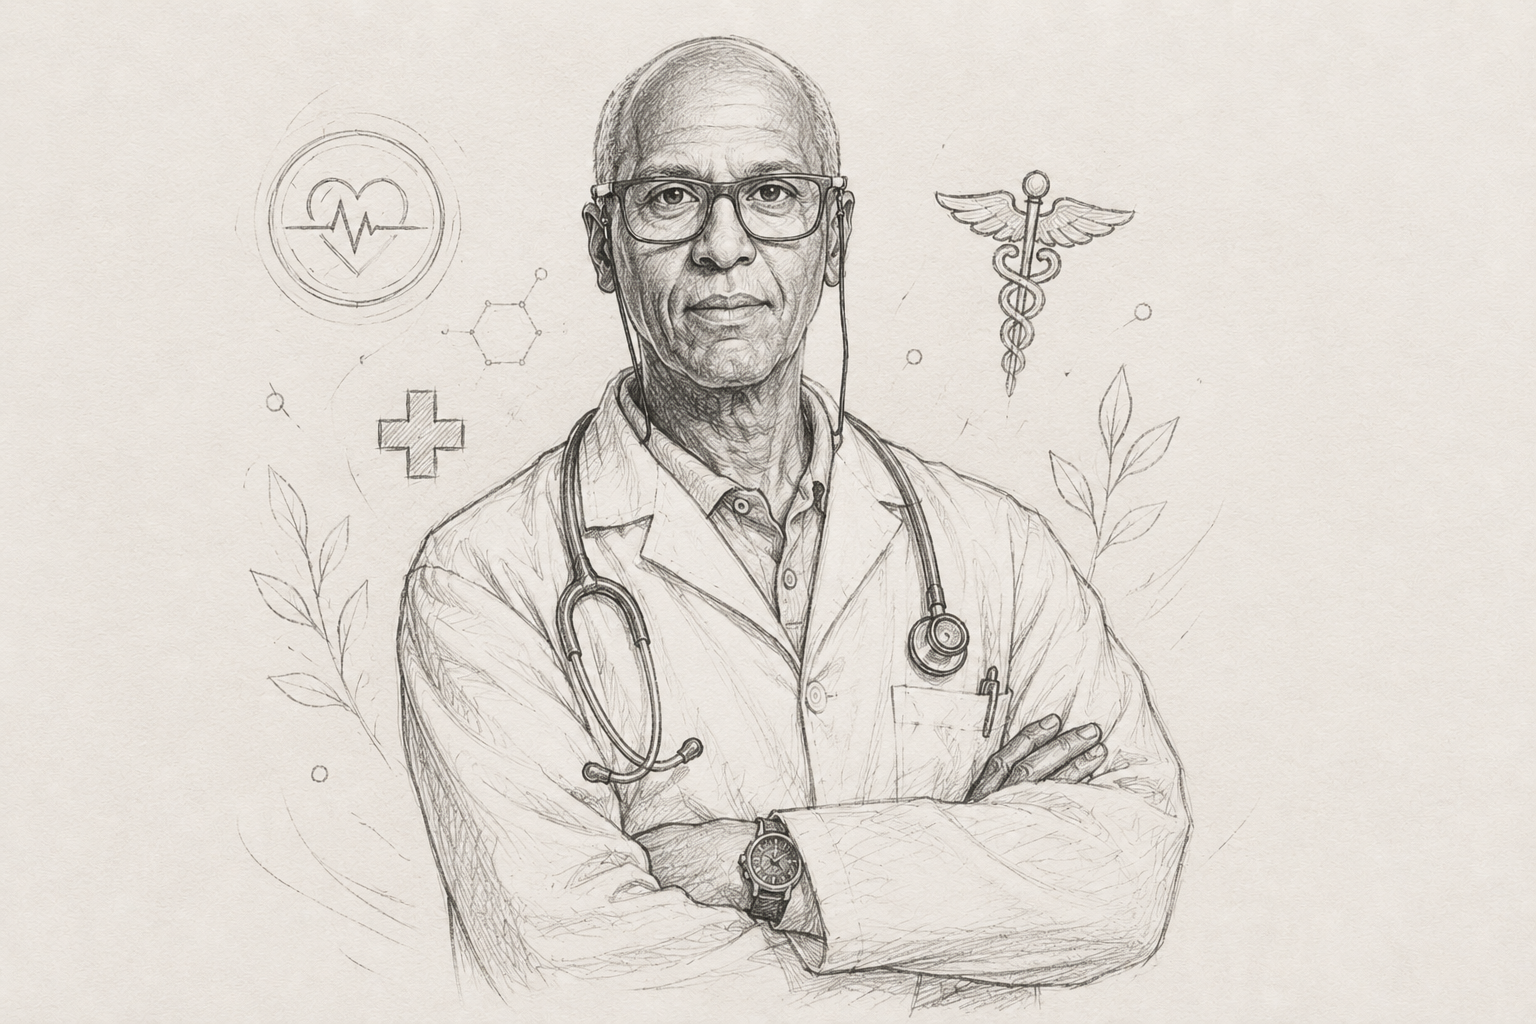
\includegraphics[width=0.85\textwidth]{../frontend/pictures/Boceto.png}
  \caption{Boceto inicial de la plataforma: mapa de secciones y primeras ideas de interfaz.}
  \label{fig:boceto}
\end{figure}

Comparando el boceto con el resultado final se aprecia que las ideas centrales sobrevivieron al desarrollo (reserva por pasos, selección de centro, identidad visual del consultorio), mientras que otras se ajustaron a lo que era posible construir con garantías en el tiempo disponible. Documentar esa evolución es parte del valor del proyecto: enseña no solo qué se hizo, sino por qué se decidió así.

\section{Metodología de desarrollo}

El proyecto no se construyó de una vez, sino de forma \textbf{iterativa e incremental}: primero una web estática que validaba la idea y la navegación, después el backend y la base de datos, luego la integración real entre frontend y API, y por último las notificaciones, la robustez para la demo y la documentación. Cada iteración partía de algo que ya funcionaba y le añadía una capa, lo que permitió detectar pronto los problemas reales —como la incoherencia entre las citas del navegador y las de la base de datos— en lugar de descubrirlos al final.

Todo el código se gestionó con \textbf{control de versiones Git}, lo que aportó un historial de cambios, la posibilidad de volver atrás ante un error y una separación clara entre lo que es código fuente y lo que son secretos o configuración local (estos últimos excluidos del repositorio mediante \texttt{.gitignore}). Se trabajó además con la distinción entre \textbf{entornos}: una configuración para desarrollo y otra preparada para producción, seleccionables por perfiles, de modo que la misma base de código se comporta de forma adecuada en cada contexto sin tocar el código. Esta forma de trabajar es, en sí misma, una de las competencias que el ciclo busca consolidar.

\section{Arquitectura general}

La solución sigue una arquitectura en capas desplegada con contenedores, de forma que cada pieza tiene una responsabilidad clara y puede sustituirse o escalarse sin arrastrar a las demás. El navegador consume el frontend (HTML, CSS y JavaScript) servido por \textbf{nginx}; las peticiones a \texttt{/api} se redirigen mediante proxy inverso al backend Java, lo que evita problemas de CORS en producción y permite presentar todo bajo un mismo origen. El backend de \textbf{Spring Boot} concentra la lógica de negocio, la seguridad y el acceso a datos sobre \textbf{PostgreSQL}, y delega en \textbf{Twilio} (servicio externo invocado desde \texttt{TwilioMessageService}) el envío de SMS y mensajes de WhatsApp. Esta separación en capas (presentación, API, persistencia y servicios externos) es la que sostiene el resto de decisiones técnicas de la memoria.

\begin{figure}[H]
\centering
\begin{tikzpicture}[node distance=1.2cm and 1.4cm, font=\small\sffamily]
  \node[block, minimum width=2.6cm] (client) {Navegador\\Paciente / Médico};
  \node[block, minimum width=2.4cm, right=of client] (nginx) {Nginx\\Frontend estático\\+ proxy \texttt{/api}};
  \node[blockaccent, minimum width=2.8cm, right=of nginx] (api) {Spring Boot 3.5\\API REST + JWT\\Java 21};
  \node[block, minimum width=2.4cm, below=of api] (db) {PostgreSQL 15\\Flyway + JPA};
  \node[block, minimum width=2.2cm, above right=0.9cm and 1.1cm of api] (twilio) {Twilio\\SMS / WhatsApp};

  \draw[arrow] (client) -- node[above, font=\scriptsize, text=graytext]{HTTPS :80} (nginx);
  \draw[arrow] (nginx) -- node[above, font=\scriptsize, text=graytext]{/api} (api);
  \draw[arrow] (api) -- node[right, font=\scriptsize, text=graytext]{JDBC} (db);
  \draw[arrow] (api) -- node[above, font=\scriptsize, text=graytext]{REST API} (twilio);

  \node[below=0.15cm of client, font=\scriptsize, text=graytext] {PWA + \texttt{service-worker.js}};
  \node[below=0.15cm of nginx, font=\scriptsize, text=graytext] {HTML/CSS/JS};
  \node[below=0.15cm of db, font=\scriptsize, text=graytext] {Perfil \texttt{postgres} o \texttt{mysql}};
\end{tikzpicture}
\caption{Arquitectura desplegada con Docker Compose (implementación actual)}
\label{fig:arquitectura}
\end{figure}


\section{Organización del backend en capas y DTOs}

Dentro del backend, el código sigue el patrón clásico de \textbf{tres capas} de Spring, con responsabilidades bien separadas:

\begin{itemize}
  \item \textbf{Controladores} (\texttt{controller}): reciben las peticiones HTTP, validan la entrada y devuelven la respuesta. No contienen lógica de negocio; solo orquestan. Ejemplos: \texttt{AuthController}, \texttt{CitaController}, \texttt{MedicoController}, \texttt{DisponibilidadController}.
  \item \textbf{Servicios} (\texttt{service}): concentran las reglas de negocio (crear una cita, comprobar disponibilidad, decidir si una cancelación es legítima) y abren las transacciones.
  \item \textbf{Repositorios} (\texttt{repository}): acceden a la base de datos mediante Spring Data JPA, incluida la consulta con bloqueo pesimista para la reserva.
\end{itemize}

Una decisión importante fue \textbf{no exponer nunca las entidades JPA directamente} en la API. Las respuestas usan objetos de transferencia de datos (\emph{DTO}) como \texttt{CitaResponse} o \texttt{ReservaPublicaResponse}, y las peticiones se modelan con clases como \texttt{CrearCitaRequest} o \texttt{ReservaPublicaRequest}. Esto tiene tres ventajas: evita filtrar al exterior campos internos o sensibles, desacopla el modelo de base de datos del contrato público de la API (se puede cambiar la entidad sin romper a los clientes) y permite validar la entrada de forma declarativa con anotaciones. Es una práctica que distingue de inmediato el código profesional del código de juguete.

\section{Stack tecnológico}

\begin{table}[H]
\centering
\caption{Componentes implementados}
\begin{tabular}{>{\bfseries\color{white}\columncolor{teal}}l >{\columncolor{white}}p{4.2cm} >{\columncolor{white}}p{5.5cm}}
\toprule
\color{white}Capa & \color{white}Tecnología & \color{white}Función \\
\midrule
Frontend & HTML5, CSS3, JS ES6+ & UI, PWA, \texttt{reserva.js} \\
\rowcolor{rowgray}
Proxy / estático & nginx (Docker) & Archivos + proxy \texttt{/api} \\
Backend & Java 21, Spring Boot 3.5.3 & API, seguridad, negocio \\
\rowcolor{rowgray}
Persistencia & PostgreSQL 15, Flyway, JPA & Datos transaccionales \\
Notificaciones & Twilio API (Java SDK) & SMS / WhatsApp \\
\rowcolor{rowgray}
Despliegue & Docker Compose & Entorno reproducible \\
Analítica & Chart.js 4 (vendorizado) & Cuadro de mando de gestión \\
\bottomrule
\end{tabular}
\end{table}

\section{Justificación de las tecnologías}

Cada pieza del stack se eligió por una razón concreta, no por moda:

\begin{itemize}
  \item \textbf{Java + Spring Boot.} El tipado fuerte de Java detecta en tiempo de compilación errores que en un lenguaje dinámico aparecerían en producción, algo especialmente valioso cuando se manejan datos de salud. Spring Boot aporta, además, un ecosistema maduro: Spring Security como estándar de facto para autenticación y autorización, Spring Data JPA para el acceso a datos y transacciones ACID que garantizan que una reserva se complete entera o no se complete en absoluto.
  \item \textbf{PostgreSQL.} Para datos críticos (usuarios, médicos, horarios y citas) hace falta integridad referencial real, transacciones fiables y bloqueo a nivel de fila. PostgreSQL ofrece las tres cosas y permite implementar el control de concurrencia con \texttt{SELECT \ldots FOR UPDATE}, núcleo de la garantía de ``no doble reserva''.
  \item \textbf{Flyway.} Versiona el esquema en migraciones numeradas (V1 a V10), de modo que cualquier entorno —el de desarrollo, el de otra persona del equipo o el de producción— se reconstruye exactamente igual al arrancar.
  \item \textbf{Twilio.} En lugar de montar infraestructura propia de mensajería, se delega el envío de SMS y WhatsApp en un proveedor consolidado, invocado directamente desde el backend Java.
  \item \textbf{Telegram (Bot API).} Se incorporó como segundo canal de aviso por una razón práctica: es gratuito y no exige que el paciente se dé de alta previamente en un \emph{sandbox}, como sí ocurre con la cuenta de prueba de Twilio. Se integra por HTTP con \texttt{RestClient}, sin SDK adicional, de modo que no añade ninguna dependencia al proyecto.
  \item \textbf{Docker Compose.} Levanta todo el sistema con un único comando, eliminando el clásico ``en mi máquina funciona''.
\end{itemize}

\section{Modelo de datos}

\begin{figure}[H]
\centering
\begin{tikzpicture}[font=\small\sffamily, node distance=0.8cm and 1.6cm]
  \node[entity, minimum width=2.4cm] (u) {\textbf{usuarios}\\\scriptsize id, email, password\\nombre, teléfono, rol};
  \node[entity, minimum width=2.2cm, right=of u] (m) {\textbf{medicos}\\\scriptsize id, nombre\\especialidad, email};
  \node[entity, minimum width=2.5cm, below=1.1cm of m] (h) {\textbf{horarios}\\\scriptsize medico\_id, inicio, fin\\disponible};
  \node[entity, minimum width=2.6cm, below=1.1cm of u] (c) {\textbf{citas}\\\scriptsize usuario\_id, medico\_id, centro\_id\\fecha\_hora, motivo, estado\\recordatorio\_enviado\\cobertura, pago (V8)};
  \node[entity, minimum width=2.5cm, right=2.2cm of c] (n) {\textbf{notificaciones}\\\scriptsize usuario\_id, cita\_id\\canal, estado\_entrega};
  \node[entity, minimum width=2.4cm, below=1.0cm of c] (ce) {\textbf{centros}\\\scriptsize codigo, nombre\\direccion, ciudad};

  \draw[rel] (u) -- node[above, sloped, font=\scriptsize]{1:N} (c);
  \draw[rel] (m) -- node[above, sloped, font=\scriptsize]{1:N} (c);
  \draw[rel] (m) -- node[right, font=\scriptsize]{1:N} (h);
  \draw[rel, dashed] (c) -- node[above, font=\scriptsize]{opc.} (n);
  \draw[rel, dashed] (u) -- (n);
  \draw[rel, dashed] (ce) -- node[right, font=\scriptsize]{opc. 1:N} (c);
  \draw[rel, dashed] (ce) to[bend left=20] node[left, font=\scriptsize]{opc. 1:N} (h);
\end{tikzpicture}
\caption{Modelo entidad-relación principal (PostgreSQL, migraciones Flyway V1--V8)}
\label{fig:er}
\end{figure}


El modelo relacional gira en torno a cuatro entidades centrales —\texttt{usuarios}, \texttt{medicos}, \texttt{horarios} y \texttt{citas}— más \texttt{notificaciones} para el registro de avisos. Un \texttt{usuario} (paciente) puede tener muchas \texttt{citas}; un \texttt{medico} tiene muchos \texttt{horarios} y muchas \texttt{citas}; cada \texttt{cita} enlaza un usuario con un médico en una fecha y hora concretas. Cada tabla cumple un papel preciso:

\begin{itemize}
  \item \texttt{usuarios}: identidad y credenciales (email único, contraseña cifrada, nombre, teléfono, rol). El campo \texttt{rol} discrimina entre \texttt{PACIENTE}, \texttt{MEDICO} y \texttt{ADMIN}, y \texttt{cuenta\_invitada} marca las cuentas creadas en una reserva sin registro. Desde la V9 guarda además el chat de Telegram vinculado (\texttt{telegram\_chat\_id}) y el token de un solo uso con el que se realiza esa vinculación.
  \item \texttt{medicos}: datos profesionales (nombre, especialidad, email de contacto del facultativo).
  \item \texttt{horarios}: la disponibilidad real, como franjas con \texttt{inicio}, \texttt{fin}, un indicador \texttt{disponible} y el centro donde se atiende (\texttt{centro\_id}, V6). Un índice único sobre \texttt{(medico\_id, inicio)} impide crear dos franjas idénticas para el mismo médico.
  \item \texttt{citas}: las reservas, que vinculan \texttt{usuario\_id} y \texttt{medico\_id} con \texttt{fecha\_hora}, \texttt{motivo} y \texttt{estado}. La cancelación no borra la fila: cambia su \texttt{estado} (mediante el enumerado \texttt{EstadoCita}), preservando la trazabilidad.
  \item \texttt{notificaciones}: el registro auditable de los avisos enviados, con su canal y estado de entrega.
  \item \texttt{centros}: los centros o consultas donde se atiende (\texttt{codigo} único, nombre, dirección, ciudad). Cada \texttt{cita} referencia opcionalmente su centro mediante \texttt{centro\_id}.
\end{itemize}

La evolución del esquema queda reflejada en las migraciones Flyway: la \texttt{V2\_\_cita\_recordatorio} añade el campo \texttt{recordatorio\_enviado} para evitar duplicar avisos Twilio, la \texttt{V3} extiende los horarios y crea el usuario médico de prueba, la \texttt{V4} introduce \texttt{cuenta\_invitada} para la reserva sin registro previo, la \texttt{V5} crea la tabla \texttt{centros} (con sus datos iniciales) y añade \texttt{centro\_id} a \texttt{citas}, la \texttt{V6} añade \texttt{centro\_id} a \texttt{horarios} (repartiendo la agenda por centro), la \texttt{V7} actualiza los centros a sus ubicaciones reales en Palma de Mallorca, la \texttt{V8} incorpora a la cita la cobertura y la preferencia de pago, la \texttt{V9} abre el canal de Telegram (\texttt{telegram\_chat\_id} y \texttt{telegram\_link\_token}, ambos con índice único) y la \texttt{V10} añade la caducidad de ese token de vinculación. Versionar el esquema de esta forma garantiza que la base de datos se construya exactamente igual en cualquier máquina.

\section{Persistencia relacional frente a NoSQL}

La elección de la base de datos no fue automática: se valoró expresamente un enfoque \textbf{NoSQL documental} (MongoDB) frente al \textbf{relacional} (PostgreSQL) antes de decidir. Ambos paradigmas son válidos, pero resuelven problemas distintos, y conviene justificar por qué uno encaja mejor en este caso.

Una base de datos documental como MongoDB brilla cuando los datos son heterogéneos y poco estructurados, cuando el esquema cambia con frecuencia y cuando se prioriza la escalabilidad horizontal sobre la consistencia inmediata; guarda documentos JSON flexibles y evita las uniones (\emph{joins}). Una base relacional, en cambio, destaca cuando los datos están fuertemente interrelacionados, cuando la integridad referencial y las transacciones \textbf{ACID} son innegociables y cuando hace falta bloqueo a nivel de fila.

En este proyecto los datos son intrínsecamente relacionales —un \texttt{usuario} reserva con un \texttt{medico} en un \texttt{horario} de un \texttt{centro}, generando una \texttt{cita}— y la invariante crítica del sistema es que \textbf{dos pacientes no reserven la misma franja}. Garantizar eso exige una transacción con bloqueo (\texttt{SELECT \ldots FOR UPDATE}), justo donde el modelo relacional es más fuerte y el documental obligaría a soluciones más artificiales. Además, el volumen de una consulta médica es modesto, de modo que la escalabilidad horizontal de NoSQL no aporta una ventaja real aquí. Por todo ello, PostgreSQL es la opción correcta para el \emph{núcleo transaccional}.

Esto no descarta NoSQL: simplemente lo reserva para donde sí encaja. El \textbf{historial clínico} es el candidato natural a un almacén documental, porque cada especialidad registra campos distintos (no hay un esquema único razonable) y los datos se añaden más que se modifican; lo mismo aplicaría a un \emph{registro de auditoría} de accesos. La evolución coherente del sistema sería, por tanto, una \textbf{persistencia políglota}: PostgreSQL para el núcleo de citas (consistencia) y MongoDB para el historial clínico (flexibilidad), una línea ya recogida entre los trabajos futuros. La decisión, en resumen, no fue ``relacional porque sí'', sino elegir la herramienta adecuada para cada tipo de dato.

\section{Frontend y paleta visual}

Los colores del documento y de los diagramas coinciden con \texttt{dr-agramonte.css}: teal principal, fondos \texttt{off-white}, tarjetas blancas y variante oscura (\texttt{data-theme="dark"}, fondo \#0F172A).

\begin{figure}[H]
\centering
\begin{tikzpicture}[node distance=0.7cm, font=\small\sffamily]
  \node[blockaccent, minimum width=3.2cm] (pages) {Páginas HTML\\index, servicios, reservar...};
  \node[block, minimum width=3cm, below=of pages] (css) {\texttt{dr-agramonte.css}\\Tema claro/oscuro\\\texttt{data-theme}};
  \node[block, minimum width=2.8cm, below left=0.6cm and 0.4cm of css] (js) {\texttt{reserva.js}\\\texttt{api-client.js}};
  \node[block, minimum width=2.6cm, below right=0.6cm and 0.4cm of css] (pwa) {Service Worker\\modo offline};

  \draw[arrow] (pages) -- (css);
  \draw[arrow] (css) -- (js);
  \draw[arrow] (css) -- (pwa);
  \node[right=0.3cm of js, font=\scriptsize, text=graytext, align=left] {Centro $\rightarrow$ calendario\\$\rightarrow$ slots API $\rightarrow$ confirmar};
\end{tikzpicture}
\caption{Capas del frontend y flujo de reserva en cuatro pasos}
\label{fig:frontend-capas}
\end{figure}


\section{Autenticación JWT}

La autenticación se resuelve con \textbf{JSON Web Tokens} en modo \emph{stateless}: el servidor no guarda sesiones en base de datos, sino que confía en un token firmado que el cliente presenta en cada petición. \texttt{AuthController} expone \texttt{POST /api/auth/login} y \texttt{POST /api/auth/registro}; al autenticarse correctamente, \texttt{JwtProvider} genera un token firmado con clave secreta (algoritmo HMAC-SHA) que incluye el identificador del usuario y una fecha de expiración. A partir de ahí, el token viaja en la cabecera \texttt{Authorization: Bearer} y \texttt{JwtAuthFilter} lo valida en cada petición protegida antes de que esta llegue al controlador.

Elegí este modelo por tres motivos concretos. Primero, \textbf{rendimiento}: al no consultar sesiones en BD, cada validación es una comprobación de firma en memoria. Segundo, \textbf{escalabilidad horizontal}: varios contenedores del backend pueden validar el mismo token sin compartir estado entre ellos. Tercero, \textbf{simplicidad de integración}: cualquier cliente (la web actual o, en el futuro, una app móvil) consume la API igual. La contrapartida honesta es que un token \emph{stateless} no se puede revocar antes de que caduque; por eso la duración es corta y la introducción de un \emph{refresh token} queda recogida como mejora futura. Las contraseñas nunca se almacenan en claro: se cifran con \texttt{BCryptPasswordEncoder} con factor de coste 12, de modo que incluso ante una fuga de la base de datos los hashes resultan costosísimos de revertir.

\section{Reserva y concurrencia}

El problema más interesante de toda la aplicación es aparentemente trivial: ¿qué pasa si dos pacientes intentan reservar la misma franja en el mismo instante? Sin control, ambos verían el hueco como libre, ambos confirmarían y el médico acabaría con dos personas citadas a la misma hora. Esto no es una hipótesis de laboratorio: en una agenda real ocurre justo en las franjas más demandadas. La solución no puede ser ``cruzar los dedos'', tiene que ser determinista.

La estrategia elegida es el \textbf{bloqueo pesimista} a nivel de base de datos. Cuando llega una reserva, el repositorio recupera el horario con un \texttt{SELECT \ldots FOR UPDATE}, que bloquea esa fila concreta hasta que termina la transacción:

\begin{lstlisting}[language=Java]
Horario horario = horarioRepository
  .findByMedicoIdAndInicioAndDisponibleTrueForUpdate(...)
  .orElseThrow(...);
\end{lstlisting}

Tras validar, se crea la \texttt{Cita} y se marca el horario como no disponible. El envío de la notificación (\texttt{CitaNotificationService}) se aplaza deliberadamente al \emph{commit} de la transacción (vía \texttt{TransactionSynchronizationManager}, fase \texttt{afterCommit}): de este modo no se mantiene el bloqueo de la fila durante la llamada de red a Twilio y, si la transacción se revierte, nunca se envía un aviso de una cita que en realidad no llegó a persistirse. El control de concurrencia es \textbf{bloqueo pesimista} (\texttt{SELECT \ldots FOR UPDATE} sobre \texttt{Horario}): si dos pacientes reservan la misma franja, una operación gana y la otra recibe \textbf{409 Conflict}, de forma determinista y sin reintentos. Esta garantía no se afirma sobre el papel: está \textbf{verificada bajo concurrencia real} —dos transacciones simultáneas en hilos distintos compitiendo por la misma franja sobre una base PostgreSQL real— como se detalla en la sección de pruebas.

\begin{figure}[H]
\centering
\begin{tikzpicture}[node distance=0.55cm, font=\small\sffamily,
  every node/.style={align=center}]
  \node[draw=teal, fill=tealpale, rounded corners=6pt, inner sep=5pt] (fe) {Frontend\\\texttt{reserva.js}};
  \node[draw=teal, fill=tealpale, rounded corners=6pt, inner sep=5pt, below=of fe] (api) {POST \texttt{/api/citas}\\JWT paciente};
  \node[draw=teal, fill=tealpale, rounded corners=6pt, inner sep=5pt, below=of api] (svc) {\texttt{CitaService.crearCita}};
  \node[draw=tealdark, fill=teal!20, rounded corners=6pt, inner sep=5pt, below=of svc] (lock) {SELECT ... FOR UPDATE\\horario disponible};
  \node[draw=teal, fill=tealpale, rounded corners=6pt, inner sep=5pt, below=of lock] (save) {INSERT cita + UPDATE horario};
  \node[draw=teallight, fill=teal!30, text=white, rounded corners=6pt, inner sep=5pt, below=of save] (tw) {Twilio: médico + paciente};

  \draw[arrow] (fe) -- (api);
  \draw[arrow] (api) -- (svc);
  \draw[arrow] (svc) -- (lock);
  \draw[arrow] (lock) -- (save);
  \draw[arrow] (save) -- (tw);
\end{tikzpicture}
\caption{Flujo de reserva de cita con bloqueo pesimista y notificaciones}
\label{fig:secuencia-reserva}
\end{figure}


\section{Reserva como invitado}

No todos los pacientes quieren —o saben— crearse una cuenta antes de pedir cita, y obligar a registrarse es una de las principales causas de abandono en cualquier formulario. Por eso la plataforma ofrece \textbf{dos vías de reserva que persisten en la misma tabla \texttt{citas}}:

\begin{itemize}
  \item \textbf{Paciente autenticado:} \texttt{POST /api/citas} con su token JWT.
  \item \textbf{Reserva pública (invitado):} \texttt{POST /api/citas/reserva-publica}, sin login previo.
\end{itemize}

En la reserva de invitado, el backend crea o reutiliza una cuenta de paciente marcada como \texttt{cuenta\_invitada} (introducida en la migración Flyway V4); la contraseña es opcional, de modo que el invitado puede ``ascender'' más adelante a cuenta completa sin perder su historial de citas. Si el email ya pertenece a una cuenta con contraseña, el sistema responde con \textbf{HTTP 409} invitando a iniciar sesión, evitando que un tercero reserve en nombre de un usuario registrado. El invitado consulta y cancela sus citas mediante su email (\texttt{GET /api/citas/por-email} y \texttt{DELETE /api/citas/publica/\{id\}}).

Es importante presentarlo con honestidad: este mecanismo es \textbf{adecuado para un prototipo}, pero en producción la consulta y cancelación por email deberían reforzarse con un enlace firmado, un código de un solo uso (OTP) o login obligatorio, para impedir que alguien acceda a las citas de otra persona conociendo solo su dirección de correo. Reconocer esa limitación forma parte del rigor del proyecto.

\paragraph{Cobertura y preferencia de pago.} A raíz del \emph{feedback} de los primeros usuarios de prueba —que echaban en falta saber el precio y los seguros aceptados antes de confirmar— el formulario de reserva captura también la \textbf{cobertura}: consulta privada, con su precio visible (80 euros), o seguro médico, con la aseguradora y el número de tarjeta sanitaria. En el caso privado se recoge además la \textbf{preferencia de pago} (en consulta u online). Estos datos se persisten en la cita mediante la migración Flyway \textbf{V8} (\texttt{cobertura}, \texttt{aseguradora}, \texttt{numero\_tarjeta\_sanitaria}, \texttt{preferencia\_pago}) y se devuelven al profesional al gestionar la agenda. El \emph{cobro} en sí no se procesa todavía: la pasarela de pago en línea se documenta como línea futura.

\section{API principal}

\begin{table}[H]
\centering
\small
\begin{tabular}{llp{6.2cm}}
\toprule
\textbf{Método} & \textbf{Ruta} & \textbf{Descripción} \\
\midrule
POST & /api/auth/login, /registro & Sesión JWT \\
GET & /api/medicos & Listado de especialistas \\
GET & /api/centros & Listado de centros / consultas \\
GET & /api/disponibilidad & Slots por médico, fecha y centro \\
POST & /api/citas & Crear cita (paciente autenticado) \\
POST & /api/citas/reserva-publica & Reserva sin login (cuenta invitada) \\
GET & /api/citas/mias & Citas del paciente (JWT) \\
GET & /api/citas/por-email & Citas del invitado por email \\
DELETE & /api/citas/\{id\} & Cancelación (paciente autenticado) \\
GET & /api/estadisticas & Cuadro de mando de gestión (rol MEDICO/ADMIN) \\
GET, POST, DELETE & /api/telegram/vinculacion & Estado, alta y baja del canal Telegram (JWT) \\
POST & /api/telegram/webhook & Lo invoca Telegram; se autentica con un secreto compartido \\
POST & /api/contact & Formulario de contacto \\
\bottomrule
\end{tabular}
\caption{Endpoints principales}
\end{table}

\section{Manejo centralizado de errores}

Una API es tan buena como sus errores: si cada fallo se devuelve de una forma distinta, el frontend se vuelve frágil y difícil de mantener. Para evitarlo, el backend usa un \texttt{GlobalExceptionHandler} que captura las excepciones de forma centralizada y las traduce a respuestas JSON consistentes, con su código HTTP adecuado. Así, una franja ya ocupada devuelve siempre \textbf{409 Conflict}, una acción sin permiso \textbf{403 Forbidden} y un recurso inexistente \textbf{404 Not Found}, todos con el mismo formato (marca de tiempo, estado, mensaje y ruta).

La ventaja es doble. Por un lado, el frontend puede confiar en una estructura de error predecible y mostrar mensajes claros al usuario (por ejemplo, ``esa hora acaba de ocuparse, elige otra'' ante un 409). Por otro, se evita filtrar trazas internas o detalles de implementación al exterior, lo que también es una cuestión de seguridad. Centralizar el manejo de errores en un único punto, en lugar de repetir bloques \texttt{try-catch} por todos los controladores, mantiene el código limpio y coherente.

\section{Notificaciones: Twilio y Telegram}

Las notificaciones son la otra mitad de la promesa del proyecto: si la web evita llamadas, tiene que avisar de forma fiable de lo que ocurre con cada cita. El envío se realiza \textbf{directamente desde el backend Java} mediante el SDK de Twilio, sin un servicio intermedio de colas. Es una arquitectura más simple y perfectamente adecuada al volumen de una consulta; un sistema de mensajería asíncrona con reintentos desacoplados sería justificable a mayor escala y se contempla como evolución futura. \texttt{CitaNotificationService} envía:
\begin{itemize}
  \item Aviso al médico (\texttt{TWILIO\_NOTIFY\_TO}) en alta y cancelación.
  \item Confirmación y cancelación al paciente, por cada canal que tenga disponible.
  \item Recordatorio $\sim$24\,h antes vía \texttt{@Scheduled} (ventana 23--25\,h).
\end{itemize}

Variables: \texttt{TWILIO\_ENABLED}, \texttt{TWILIO\_ACCOUNT\_SID}, \texttt{TWILIO\_AUTH\_TOKEN}, \texttt{TWILIO\_FROM}, \texttt{TWILIO\_CHANNEL} (whatsapp o sms).

\paragraph{El segundo canal: un bot de Telegram.} La cuenta de prueba de Twilio impone una limitación incómoda para un producto real: el paciente debe darse de alta en el \emph{sandbox} antes de poder recibir nada, y los mensajes salientes tienen coste. Por eso se añadió un \textbf{segundo canal independiente} sobre la \emph{Bot API} de Telegram, que es gratuita y no exige alta previa. La integración es deliberadamente ligera —una llamada HTTP con \texttt{RestClient} a \texttt{sendMessage}, sin SDK ni dependencias nuevas— y vive en \texttt{TelegramMessageService}, gemelo de \texttt{TwilioMessageService}.

El punto interesante no es el envío, sino \textbf{cómo se averigua a qué chat escribir}. Telegram no permite iniciar una conversación con alguien: es el usuario quien tiene que escribir primero al bot. El flujo implementado resuelve ese problema con un enlace profundo y un token de un solo uso:
\begin{enumerate}
  \item El paciente, con su sesión iniciada, pulsa \emph{Recibir avisos por Telegram}. El backend (\texttt{TelegramVinculacionService}) genera un token de 32 bytes con \texttt{SecureRandom}, lo guarda en su fila de \texttt{usuarios} con una caducidad de 15 minutos y devuelve el enlace \texttt{https://t.me/<bot>?start=<token>}.
  \item Al abrirlo, Telegram envía al bot el mensaje \texttt{/start <token>}, que llega al backend a través del \emph{webhook} \texttt{POST /api/telegram/webhook}.
  \item El controlador busca al dueño de ese token, comprueba que no haya caducado, asocia el \texttt{chat\_id} a su cuenta y \textbf{consume el token} (lo pone a \texttt{NULL}). A partir de ese momento, ese paciente recibe por Telegram los mismos avisos que por SMS.
\end{enumerate}

Hay dos decisiones de seguridad que conviene subrayar. La primera: el token \textbf{se emite siempre para el usuario del JWT}, nunca para un correo recibido por parámetro; de lo contrario cualquiera podría solicitar el token de otra persona y desviar a su propio chat los avisos de las citas ajenas. La segunda: como la ruta del \emph{webhook} es pública —Telegram no puede presentar un JWT—, se autentica con el secreto compartido que se registra en \texttt{setWebhook} y que Telegram devuelve en la cabecera \texttt{X-Telegram-Bot-Api-Secret-Token}, comparado en tiempo constante. Superada esa verificación, el \emph{webhook} responde siempre \texttt{200 OK} aunque el contenido no sirva, porque un error haría que Telegram reintentase el mismo mensaje indefinidamente.

Ambos canales son \textbf{independientes y opcionales}: se activan por variables de entorno (\texttt{TELEGRAM\_ENABLED}, \texttt{TELEGRAM\_BOT\_TOKEN}, \texttt{TELEGRAM\_BOT\_USERNAME}, \texttt{TELEGRAM\_WEBHOOK\_SECRET}) y ninguno de los dos puede tumbar una reserva: los servicios de mensajería nunca propagan la excepción hacia el flujo de citas, solo registran el fallo y devuelven \texttt{false}. Si un canal está caído o apagado, el otro sigue avisando. El paciente puede además retirar el canal en cualquier momento (\texttt{DELETE /api/telegram/vinculacion}), lo que borra su \texttt{chat\_id}: una forma concreta de aplicar el derecho de supresión del RGPD.

\section{Implementación del frontend}

El frontend se construyó con HTML5, CSS3 y JavaScript nativo, sin frameworks como React o Vue. No fue la primera idea: al principio valoré usar React o incluso Python en el cliente, en parte por mi formación y por el \emph{feedback} de profesionales del sector (OmniAccess). Sin embargo, tras un análisis de necesidades reales del proyecto, decidí prescindir de esa maquinaria. Fue una decisión consciente de ingeniería: la aplicación no maneja un estado global tan complejo como para justificarla, y evitarla reduce dependencias, acelera la carga inicial y permite que cualquier persona lea y modifique el código sin aprender antes una librería ni arrastrar un \texttt{node\_modules} de cientos de megas. El JavaScript se organiza en módulos reutilizables (\texttt{api-client.js} para las llamadas REST con JWT, y la lógica de reserva en \texttt{reserva.js}), lo que evita duplicar código entre páginas. Saber \emph{cuándo no} añadir una tecnología es, para un perfil de desarrollo, tan importante como saber usarla.

\begin{itemize}
  \item \textbf{Reserva:} \texttt{reservar.html} + \texttt{reserva.js} (centros, calendario, franjas desde la API y \emph{fallback} local).
  \item \textbf{Servicios:} los enlaces \texttt{reservar.html?servicio=...} preconfiguran tipo de consulta y motivo.
  \item \textbf{Tema:} botón luna/sol con preferencia recordada, y clase \texttt{btn--reserva} unificada en todo el sitio.
  \item \textbf{PWA:} \texttt{manifest.json} y \texttt{service-worker.js}; página \texttt{offline.html} para cuando no hay conexión.
\end{itemize}

\paragraph{Aplicación web progresiva (PWA).} La web es instalable en el móvil como si fuera una app, sin pasar por una tienda de aplicaciones. Esto se logra con tres piezas: un \texttt{manifest.json} que define nombre, iconos y color de tema; un \emph{service worker} que cachea los recursos críticos para que la navegación siga funcionando aunque la conexión falle, mostrando una página \texttt{offline.html} cuando no hay red; y el requisito de servir bajo HTTPS en producción. Para un paciente, la diferencia práctica es poder tener ``Dr. Agramonte'' como un icono más en su pantalla de inicio, reforzando justamente la idea de un canal propio y cercano al consultorio.

\paragraph{Selección de centro (multi-ubicación).} El flujo de reserva permite elegir entre dos centros antes de fijar la hora: \emph{Consulta General Riera} y \emph{Consulta Avenidas}, ambos en Palma de Mallorca y cada uno con sus propios días de atención. Esto refleja una realidad habitual: un mismo profesional atiende en más de una ubicación. El centro \textbf{se persiste en la base de datos}: existe una entidad \texttt{Centro} (tabla \texttt{centros}, creada en la migración Flyway V5) con un \texttt{codigo} estable —\texttt{madrid}, \texttt{palma}— que coincide con el identificador que ya empleaba el frontend, de modo que no hubo que reescribir la web. El backend expone el listado mediante \texttt{GET /api/centros}.

\paragraph{Agenda del médico por centro.} La multi-ubicación se llevó hasta el final: cada \texttt{horario} pertenece a un centro (columna \texttt{centro\_id}, migración V6; la V7 actualizó los centros a sus ubicaciones reales en Palma de Mallorca), repartiendo la agenda del médico por día de la semana —la consulta de General Riera los lunes, martes y jueves; la de Avenidas los miércoles, viernes y sábados— de forma que cada día el profesional está en un único sitio. A partir de ahí, todo encaja de manera coherente:
\begin{itemize}
  \item La \textbf{disponibilidad se filtra por centro}: \texttt{GET /api/disponibilidad?medicoId=\&fecha=\&centroCodigo=} solo devuelve los huecos de ese centro (un miércoles no ofrece horas de General Riera).
  \item La \textbf{cita hereda el centro de su horario}: al reservar, el centro no se deduce de lo que diga el cliente, sino de la franja realmente reservada, lo que evita incoherencias.
  \item La \textbf{agenda del médico muestra el centro} de cada cita y puede filtrarse por ubicación.
\end{itemize}
Todas las relaciones con \texttt{centro} son \emph{nullable} a propósito: las citas y horarios anteriores a esta funcionalidad siguen siendo válidos.

\paragraph{Reserva guiada por pasos.} La experiencia se divide en pasos pequeños (centro $\rightarrow$ calendario $\rightarrow$ hora $\rightarrow$ datos $\rightarrow$ confirmación) para reducir la carga cognitiva y no abrumar al usuario con todos los campos a la vez. Esta decisión, heredada del boceto inicial, es especialmente importante para pacientes mayores o poco habituados a la tecnología.

\paragraph{Accesibilidad.} La interfaz cuida el uso de etiquetas HTML semánticas, atributos ARIA, un orden de tabulación lógico para navegar solo con teclado y un contraste de color suficiente entre texto y fondo, tanto en modo claro como oscuro. La accesibilidad no se entendió como un requisito formal, sino como la diferencia entre que una persona mayor pueda usar la aplicación o no. Por su importancia en un contexto sanitario, se detalla en su propia sección a continuación.

\paragraph{Validación de datos.} La entrada del usuario se valida en dos niveles, porque ninguno de los dos basta por sí solo. En el \textbf{frontend} se comprueban formato de email, teléfono español y campos obligatorios antes de enviar, dando un aviso inmediato y evitando viajes innecesarios al servidor; esto mejora la experiencia, pero no es una garantía de seguridad porque puede manipularse. Por eso la validación se repite en el \textbf{backend} con las anotaciones de \emph{Bean Validation} sobre los DTO de entrada: el servidor nunca confía en que el cliente haya validado bien. Esta doble barrera —comodidad en el cliente, seguridad en el servidor— es un principio básico de cualquier aplicación web seria.

\section{Accesibilidad y usabilidad (WCAG)}

En una aplicación de salud, la accesibilidad no es un extra: una parte importante de los pacientes son personas mayores o con dificultades visuales o motrices, y si no pueden usar la herramienta, esta sencillamente no cumple su función. Por eso la interfaz se diseñó tomando como referencia las \textbf{Pautas de Accesibilidad para el Contenido Web (WCAG 2.1)} en su nivel \textbf{AA}, organizadas en torno a sus cuatro principios: perceptible, operable, comprensible y robusto.

\paragraph{Perceptible: contraste de color verificado.} El contraste entre texto y fondo se comprobó con la fórmula de luminancia relativa de la WCAG, no a ojo. El texto principal y los elementos interactivos superan con holgura el umbral AA de 4{,}5:1 para texto normal. Durante la revisión se detectó que el gris más claro usado para textos secundarios se quedaba en 2{,}5:1 (no cumplía) y se oscureció hasta cumplir, manteniendo en el modo oscuro un tono claro que conserva el contraste sobre fondo oscuro. La tabla siguiente recoge las medidas reales tras el ajuste:

\begin{table}[H]
\centering
\small
\caption{Ratios de contraste medidos (modo claro, sobre fondo blanco)}
\begin{tabular}{lcc}
\toprule
\textbf{Uso} & \textbf{Ratio} & \textbf{WCAG AA} \\
\midrule
Texto principal (gris oscuro) & 14{,}7:1 & \checkmark \\
Botones (blanco sobre teal) & 5{,}5:1 & \checkmark \\
Enlaces y acentos (teal) & 5{,}5:1 & \checkmark \\
Texto secundario (gris medio) & 4{,}8:1 & \checkmark \\
Texto auxiliar / hints (ajustado) & 4{,}6:1 & \checkmark \\
Mensajes de error (rojo) & 4{,}8:1 & \checkmark \\
\bottomrule
\end{tabular}
\end{table}

\paragraph{Operable: teclado y navegación.} Toda la aplicación se puede manejar solo con teclado, con un orden de tabulación lógico y un \textbf{foco visible} reforzado (un contorno claro con \texttt{:focus-visible} de 2\,px sobre cada elemento al recibir el foco). Se añadió además un \textbf{enlace para saltar al contenido} (``Ir al contenido principal''), oculto hasta que recibe el foco, que permite a quien navega con teclado o lector de pantalla evitar la cabecera repetida en cada página y llegar directamente al contenido; esto cubre el criterio WCAG 2.4.1 (\emph{Evitar bloques}). El flujo de reserva se divide en pasos cortos para exigir los mínimos clics posibles y no abrumar.

\paragraph{Comprensible: estructura y ayuda.} El marcado es HTML semántico (encabezados jerárquicos, \texttt{nav}, \texttt{main}, \texttt{footer}), con el idioma declarado (\texttt{lang="es"}) para que los lectores de pantalla lo pronuncien correctamente, atributos ARIA donde el componente lo requiere y una etiqueta asociada a cada campo de formulario. La validación de los datos es inmediata y con mensajes claros, y la reserva guiada por pasos reduce la carga cognitiva, algo especialmente valioso para usuarios poco habituados a la tecnología.

\paragraph{Robusto: preferencias del usuario y zoom.} La maquetación usa unidades relativas (\texttt{rem}, \texttt{clamp}) que permiten ampliar el tamaño de letra del navegador sin que la interfaz se rompa, y respeta la preferencia del sistema \texttt{prefers-reduced-motion}, desactivando las animaciones para quienes sufren mareo con el movimiento (problemas vestibulares). El modo claro/oscuro, además de comodidad, ofrece una alternativa a personas sensibles al brillo.

\paragraph{Limitación honesta.} La accesibilidad se ha trabajado por diseño y se ha verificado el contraste de forma manual, pero no se ha pasado todavía una auditoría automática completa (por ejemplo, \emph{Lighthouse} o \emph{axe}) ni se ha probado con usuarios reales de lector de pantalla. Documentar esa auditoría y realizar pruebas con usuarios es la evolución natural de este apartado, ya recogida entre las líneas futuras de calidad.

\section{Sincronización de citas: una sola fuente de verdad}

Uno de los problemas más instructivos del desarrollo no fue de algoritmos, sino de \emph{coherencia de datos} entre vistas. Al principio, la lista ``Mis citas programadas'' que veía el paciente vivía solo en el \texttt{localStorage} del navegador, mientras que el panel de pruebas del médico leía de la base de datos. El resultado eran incoherencias desconcertantes: citas que aparecían para el paciente pero no en el panel, cancelaciones que solo existían en un navegador, e incluso reservas antiguas con identificadores locales que nunca habían llegado al servidor.

La solución fue establecer una \textbf{única fuente de verdad}: PostgreSQL. La función \texttt{syncMisCitas()} de \texttt{reserva.js} sustituye la caché local por lo que realmente hay en el servidor, consultando \texttt{GET /api/citas/mias} para el paciente autenticado o \texttt{GET /api/citas/por-email} para el invitado. Esta sincronización se dispara en los momentos clave: al cargar la página de reserva, tras confirmar o cancelar una cita, al escribir el email (con \emph{debounce}) y tras iniciar o cerrar sesión. Así, lo que ve el paciente y lo que ve el panel siempre coinciden, porque ambos derivan del mismo origen. La regla de diseño es sencilla: \emph{el navegador nunca es la verdad; solo refleja la base de datos tras cada sincronización.}

\section{Cuadro de mando de gestión (analítica)}

Una consulta médica no es solo una agenda: es una pequeña empresa que genera datos cada día. Esos datos, si se quedan dispersos en filas de una tabla, no le dicen nada al profesional; pero agregados y representados visualmente revelan información útil para tomar decisiones: qué especialidad se demanda más, cómo se reparte la carga de trabajo, qué centro concentra más actividad o cuántas citas se cancelan. Con esa idea —entender la clínica como un negocio que se puede medir y optimizar— se incorporó un \textbf{cuadro de mando de gestión}, accesible solo para el personal interno.

La pieza clave es que toda la analítica se calcula \textbf{en la base de datos}, no en memoria. El endpoint \texttt{GET /api/estadisticas} se apoya en consultas de agregación \texttt{GROUP BY} (con \texttt{COUNT}, \texttt{JOIN}, \texttt{LEFT JOIN}, \texttt{COALESCE} para los valores nulos y las funciones de fecha \texttt{YEAR()}/\texttt{MONTH()}) que devuelven directamente los totales ya calculados. Para no traer las entidades completas a memoria, cada consulta usa una \emph{proyección} ligera de Spring Data —una interfaz con solo los campos necesarios (etiqueta y total)—, lo que mantiene la respuesta pequeña y la consulta eficiente. El servicio que orquesta estas consultas se marca como \texttt{@Transactional(readOnly = true)}, una señal explícita de que solo lee datos y nunca los modifica. El cálculo de indicadores derivados, como la tasa de cancelación, se hace en el servicio a partir del reparto por estado, evitando consultas redundantes.

El cuadro de mando presenta primero cuatro indicadores resumen (KPIs) y, debajo, cinco gráficos:

\begin{itemize}
  \item \textbf{Indicadores:} total de citas, citas activas (pendientes y confirmadas), completadas y \textbf{tasa de cancelación} como aproximación al ausentismo.
  \item \textbf{Carga de trabajo por médico} (barras): cuántas citas gestiona cada facultativo, de mayor a menor.
  \item \textbf{Demanda por especialidad} (barras): las áreas más solicitadas.
  \item \textbf{Distribución por centro} (barras): el reparto de actividad entre ubicaciones.
  \item \textbf{Reparto por estado} (anillo): la proporción de confirmadas, pendientes, completadas y canceladas.
  \item \textbf{Evolución temporal} (línea): el volumen de citas mes a mes, para detectar tendencias.
\end{itemize}

En el frontend, los gráficos se dibujan con \textbf{Chart.js}, una librería ligera que se incorporó \emph{vendorizada} en el propio repositorio (\texttt{js/vendor/}) en lugar de cargarse desde una CDN externa. La decisión es deliberada: el sistema no depende de una conexión a internet ajena para funcionar —coherente con la filosofía PWA y \emph{offline first} del proyecto— y la aplicación se puede mostrar aunque no haya red. La página respeta el modo claro/oscuro recalculando los colores al cambiar de tema, y \textbf{degrada con elegancia}: si quien la abre no ha iniciado sesión como personal autorizado, en lugar de un error muestra un aviso claro invitando a identificarse.

El acceso está restringido en \texttt{SecurityConfig} a los roles \texttt{MEDICO} y \texttt{ADMIN}: las analíticas de negocio son una herramienta interna y no deben ser visibles para un paciente ni para un usuario anónimo. Esta restricción se verificó en vivo —una petición sin token recibe \textbf{403 Forbidden}, mientras que con el token de un médico el endpoint devuelve los datos agregados—, lo que conecta este módulo directamente con la política de autorización por rol descrita más adelante. En conjunto, el cuadro de mando demuestra la competencia de \emph{sistemas de gestión empresarial}: convertir los datos operativos del día a día en información de gestión accionable.

\section{Seguridad y RGPD}

La seguridad no se añadió al final, se diseñó desde el principio, porque manejar datos de salud obliga a ello. El acceso está gobernado por roles (\texttt{PACIENTE}, \texttt{MEDICO}, \texttt{ADMIN}) declarados en \texttt{SecurityConfig}: cada ruta exige el rol mínimo necesario, de modo que un paciente no puede asomarse a la agenda del médico ni un usuario anónimo crear citas en nombre de otro. Sobre esa base se aplican las medidas concretas de protección de datos:

\begin{itemize}
  \item Contraseñas con \texttt{BCryptPasswordEncoder(12)}.
  \item CORS configurado para orígenes de desarrollo y producción.
  \item Política de privacidad en \texttt{privacidad.html} y checkbox de aceptación en el formulario de reserva.
  \item Secretos (\texttt{JWT\_SECRET}, Twilio, token del bot de Telegram) en \texttt{.env}, no en el repositorio.
  \item \textbf{Webhook público autenticado:} la ruta que invoca Telegram no puede presentar un JWT, así que se valida con el secreto compartido que se registra en \texttt{setWebhook} y que Telegram reenvía en cada llamada; la comparación se hace en \textbf{tiempo constante} (\texttt{MessageDigest.isEqual}) para no filtrar información por el tiempo de respuesta.
  \item \textbf{Análisis de vulnerabilidades:} \texttt{OWASP dependency-check} configurado en \texttt{pom.xml}, que hace fallar el build con CVSS\,$\geq$\,7.
\end{itemize}

\section{Despliegue}

Uno de los objetivos era que el sistema completo se pudiera levantar sin instalar nada manualmente, ni siquiera por alguien sin experiencia previa. Por eso todo el despliegue se reduce a un único comando, que construye las imágenes y arranca los contenedores en el orden correcto:

\begin{lstlisting}[language=bash]
docker compose up -d --build
\end{lstlisting}

Esto levanta tres servicios coordinados: \texttt{postgres} (la base de datos), \texttt{backend} en el puerto 8080 (la API Spring Boot) y \texttt{frontend} en el puerto 80 (nginx sirviendo la web y haciendo de proxy de \texttt{/api}). El \texttt{docker-compose} define dependencias y comprobaciones de salud, de modo que el backend no se da por listo hasta que la base de datos responde. El artefacto del backend es un \textbf{JAR de Spring Boot con servidor embebido} (generado por \texttt{spring-boot-maven-plugin}), el esquema de la base de datos se versiona con Flyway —que aplica las migraciones pendientes en el primer arranque— y la configuración se separa por perfiles (\texttt{application-postgres.yml} y \texttt{application-mysql.yml}), existiendo además un perfil opcional de MySQL con \texttt{--profile mysql}. La ventaja práctica es enorme: cualquier entorno queda idéntico al de desarrollo, eliminando el clásico ``en mi máquina funciona''.

\paragraph{Dominio e identidad de marca.} De cara al salto a producción se ha registrado el dominio \textbf{\texttt{dragramonte.com}}, una marca personal corta, profesional y fácil de dictar por teléfono (frente a alternativas más largas que se descartaron). La aplicación ya está preparada para ese dominio: los pies de página, la página de contacto, las etiquetas \texttt{Open Graph} y la política de CORS del backend apuntan a \texttt{dragramonte.com}, y el correo de contacto utiliza la propia marca (\texttt{contacto@dragramonte.com}). El despliegue, además, ya está \textbf{en producción}: la aplicación se ejecuta en un \textbf{servidor propio (VPS) con Docker}, empaquetada con un \texttt{Dockerfile} \emph{multi-stage} en el que el backend Spring Boot sirve a la vez la API y el frontend en un \textbf{único contenedor} —junto a un PostgreSQL que solo escucha en la red interna—, con \textbf{Caddy} como proxy inverso delante, y es \textbf{accesible públicamente con HTTPS} (certificado Let's Encrypt, renovado de forma automática) en \url{https://www.dragramonte.com}. Llegar a un dominio propio, con certificado válido y la aplicación abierta a cualquier navegador, es una madurez poco habitual en un proyecto de este tamaño; la migración de identidad de marca ya estaba hecha en el código y ahora se acompaña del despliegue real.

\section{Sostenibilidad y eficiencia (green computing)}

La sostenibilidad de este proyecto no es una etiqueta añadida al final, sino una consecuencia directa de las decisiones de diseño. Un software es sostenible cuando consume los recursos justos —energía, ancho de banda, hardware y, en última instancia, dinero— para hacer su trabajo, y cuando además \emph{sustituye} procesos físicos más costosos. Dr.\ Agramonte actúa en los dos frentes: reduce el gasto material de la consulta y se ha construido para gastar poco al ejecutarse.

\paragraph{Digitalización y ahorro de papel.} El primer impacto es el más evidente: la aplicación elimina la agenda de papel y los apuntes manuales que hoy usan muchas consultas pequeñas. Las citas, sus cambios y su historial viven en la base de datos, y los avisos llegan por canales digitales (SMS o WhatsApp vía Twilio) en lugar de recordatorios impresos o llamadas que consumen tiempo y, a veces, desplazamientos. Menos papel significa menos impresión, menos almacenamiento físico y menos residuos; y al evitar visitas o llamadas innecesarias para gestionar una cita, se reduce también el desplazamiento del paciente, con su correspondiente huella. Es la traducción concreta del objetivo de desarrollo sostenible \textbf{ODS 12} (producción y consumo responsables) a una consulta médica.

\paragraph{Software eficiente, menos energía.} La eficiencia técnica es, en la práctica, eficiencia energética: cada ciclo de CPU y cada byte transferido que se ahorran se traducen en menos consumo, tanto en el servidor como en los miles de dispositivos de los pacientes. Varias decisiones del proyecto van en esa dirección:
\begin{itemize}
  \item \textbf{Frontend sin framework.} Prescindir de React o Vue evita arrastrar un \texttt{node\_modules} de cientos de megas y enviar grandes paquetes de JavaScript al navegador. La web carga más rápido y exige menos CPU al cliente, lo que en un parque grande de dispositivos no es despreciable.
  \item \textbf{Recursos vendorizados.} Servir Chart.js desde el propio dominio en lugar de una CDN externa reduce peticiones de red a terceros y dependencias innecesarias.
  \item \textbf{Cálculo en la base de datos.} El cuadro de mando agrega los datos con consultas \texttt{GROUP BY} en PostgreSQL en lugar de traer todas las filas a memoria y procesarlas en la aplicación. Mover el cálculo a donde están los datos transfiere menos información y gasta menos memoria y CPU en el backend.
  \item \textbf{Una sola base de datos relacional.} No hay un clúster de servicios (Redis, Mongo) corriendo y consumiendo energía en reposo: un único PostgreSQL cubre las necesidades reales del volumen de una consulta.
  \item \textbf{Autenticación \emph{stateless}.} El token JWT evita guardar sesiones en el servidor, reduciendo el estado que hay que almacenar y mantener.
\end{itemize}

\paragraph{Infraestructura ligera y escalable a la baja.} El backend se empaqueta con un \texttt{Dockerfile} \emph{multi-stage}, de modo que la imagen final solo contiene el JRE y el JAR, sin las herramientas de compilación: imágenes más pequeñas significan menos disco, descargas más rápidas y menos energía en cada despliegue. El sistema completo cabe holgadamente en un servidor modesto (un VPS pequeño basta para una consulta), y los contenedores pueden apagarse cuando no se usan. Frente a la tendencia de sobredimensionar (\emph{just in case}), aquí se dimensiona para la necesidad real (\emph{just enough}), que es la forma más directa de \textbf{green computing}: no encender lo que no hace falta.

\paragraph{Sostenibilidad del propio software.} Un sistema también es sostenible si dura. La reproducibilidad con Docker y Flyway evita reconstrucciones manuales propensas a error; el análisis de vulnerabilidades con OWASP \texttt{dependency-check} mantiene las dependencias sanas en el tiempo; y un código legible, sin capas innecesarias, es más fácil de mantener durante años por otra persona. Un software que se mantiene vivo y seguro no hay que reescribirlo desde cero cada poco, lo que es una forma de no malgastar esfuerzo ni recursos.

\paragraph{Limitación honesta.} No se ha realizado una medición formal de la huella de carbono ni del consumo energético real (con herramientas como auditorías de \emph{Lighthouse} o medidores de consumo del contenedor); las afirmaciones anteriores son cualitativas y se apoyan en las decisiones de arquitectura, no en métricas instrumentadas. Cuantificar ese ahorro —por ejemplo, comparar el consumo del frontend frente a una versión con framework— es una línea de mejora natural y coherente con el resto del proyecto.

\section{Planificación temporal}

El desarrollo se organizó en fases encadenadas a lo largo de cuatro meses, partiendo del análisis y el diseño de datos antes de escribir el grueso del backend, y dejando la redacción de la memoria como una tarea transversal que acompañó a todo el proyecto. El diagrama de Gantt de la figura siguiente resume esa planificación por hitos; en la práctica algunas fases se solaparon (por ejemplo, las pruebas se fueron escribiendo a la vez que avanzaban backend y frontend), algo habitual y deseable en un desarrollo iterativo.

\begin{center}
\begin{tikzpicture}[x=0.45cm, y=0.55cm, font=\scriptsize\sffamily]
  \draw[very thin, bordergray] (0,0) grid (24,8);
  \foreach \x/\txt in {2/M1, 8/M2, 14/M3, 20/M4}
    \node at (\x+1,8.6) [font=\bfseries, text=tealdark] {\txt};
  \node[left, text=tealdark] at (0,7) {Análisis};
  \node[left, text=tealdark] at (0,6) {Diseño BD/API};
  \node[left, text=tealdark] at (0,5) {Backend};
  \node[left, text=tealdark] at (0,4) {Frontend};
  \node[left, text=tealdark] at (0,3) {Twilio + pruebas};
  \node[left, text=tealdark] at (0,2) {Docker};
  \node[left, text=tealdark] at (0,1) {Memoria};
  \fill[teal] (0,6.7) rectangle (4,7.3);
  \fill[tealdark] (3,5.7) rectangle (7,6.3);
  \fill[teal] (6,4.7) rectangle (13,5.3);
  \fill[teallight] (12,3.7) rectangle (18,4.3);
  \fill[teal] (11,2.7) rectangle (16,3.3);
  \fill[tealdark] (17,1.7) rectangle (21,2.3);
  \fill[tealpale, draw=teal] (18,0.7) rectangle (24,1.3);
\end{tikzpicture}
\captionof{figure}{Diagrama de Gantt por hitos (M1--M4).}
\end{center}

\section{Pruebas y validación}

La estrategia de pruebas se centró en los \textbf{caminos críticos}, aquellos en los que un fallo tendría consecuencias reales: la no duplicación de reservas, el respeto de los permisos por rol y la validez del token de autenticación. La filosofía no fue ``probarlo todo'' de forma superficial, sino probar bien lo que importa, combinando tres niveles —unitario, de seguridad e integración— para cubrir el comportamiento desde distintos ángulos. El proyecto incorpora una batería de \textbf{47 pruebas automatizadas}, ejecutable con \texttt{mvn test} desde \texttt{backend/}:

\begin{itemize}
  \item \textbf{Unitarias (caja blanca):} \texttt{CitaServiceTest} (reserva sobre franja libre confirma y bloquea el horario; franja ocupada $\rightarrow$ 409 sin persistir; cancelación por no propietario $\rightarrow$ 403; re-cancelación $\rightarrow$ 409). \texttt{JwtProviderTest} (generación, validación y expiración del token firmado). \texttt{TelegramVinculacionServiceTest} (el token de vinculación se emite con caducidad, dos llamadas seguidas no repiten token, uno caducado no cuenta como vinculación pendiente, la desvinculación es idempotente y con el canal apagado la petición responde 503).
  \item \textbf{Seguridad / RBAC (caja negra, WebMvc):} \texttt{CitaControllerWebMvcTest} importa la \texttt{SecurityConfig} real: rol MEDICO sobre rutas de paciente $\rightarrow$ 403; acceso anónimo bloqueado; rol PACIENTE $\rightarrow$ 201. \texttt{TelegramVinculacionControllerWebMvcTest} comprueba que las tres operaciones del canal exigen sesión y que siempre actúan sobre el usuario del \emph{principal}, nunca sobre uno indicado por parámetro. \texttt{TelegramWebhookControllerWebMvcTest} cubre la ruta pública del \emph{webhook}: sin la cabecera del secreto o con un secreto que no coincide $\rightarrow$ 401 sin tocar la base de datos; con el secreto correcto, \texttt{/start <token>} vincula el chat; y un token caducado no vincula.
  \item \textbf{Integración end-to-end (Testcontainers + PostgreSQL real):} \texttt{ReservaPublicaIntegrationTest}: \emph{(a)} \textbf{concurrencia real}: dos transacciones simultáneas, en hilos distintos sincronizados con una \texttt{CyclicBarrier}, compiten por la misma franja; exactamente una confirma (201) y la otra recibe 409, demostrando el bloqueo pesimista sobre PostgreSQL —algo que un H2 en memoria no reproduce y que un \emph{mock} no prueba—; \emph{(b)} segunda reserva secuencial sobre la franja ya ocupada $\rightarrow$ 409; \emph{(c)} reserva pública persistida y consultable por email; \emph{(d)} agenda por centro: el hueco se filtra por ubicación y la cita hereda el centro del horario.
  \item \textbf{Análisis de vulnerabilidades:} \texttt{OWASP dependency-check} (\texttt{mvn org.owasp:dependency-check-maven:check}).
  \item \textbf{Manuales:} compilación Maven, arranque Docker Compose y health check; flujo registro/login $\rightarrow$ reservar $\rightarrow$ mis citas $\rightarrow$ cancelar; parámetro \texttt{?servicio=}; validación de formularios (email, teléfono español).
\end{itemize}

\begin{table}[H]
\centering
\small
\caption{Matriz de trazabilidad requisito $\leftrightarrow$ prueba (RTM)}
\begin{tabular}{llll}
\toprule
\textbf{Requisito} & \textbf{Prueba} & \textbf{Tipo} & \textbf{Resultado} \\
\midrule
No doble reserva (2 hilos a la vez) & \texttt{ReservaPublicaIntegrationTest} & Integración & 201/409 \checkmark \\
\rowcolor{rowgray}
RBAC / menor privilegio & \texttt{CitaControllerWebMvcTest} & Seguridad & 403 \checkmark \\
JWT firmado válido & \texttt{JwtProviderTest} & Unitaria & \checkmark \\
\rowcolor{rowgray}
Solo el dueño cancela & \texttt{CitaServiceTest} & Unitaria & 403 \checkmark \\
No re-cancelar & \texttt{CitaServiceTest} & Unitaria & 409 \checkmark \\
\rowcolor{rowgray}
Webhook público sin secreto válido & \texttt{TelegramWebhookControllerWebMvcTest} & Seguridad & 401 \checkmark \\
\rowcolor{rowgray}
Canal Telegram solo del propio usuario & \texttt{TelegramVinculacionControllerWebMvcTest} & Seguridad & 401/204 \checkmark \\
Token de vinculación caducado & \texttt{TelegramVinculacionServiceTest} & Unitaria & \checkmark \\
\bottomrule
\end{tabular}
\end{table}

\paragraph{Requisito de las pruebas de integración.} Las cinco pruebas de \texttt{ReservaPublicaIntegrationTest} levantan un PostgreSQL real mediante Testcontainers y, por tanto, necesitan un motor Docker en marcha. Cuando no lo hay, la propia suite las marca como \emph{saltadas} en lugar de fallar, de modo que \texttt{mvn test} sigue siendo verde en una máquina sin Docker; para una verificación completa conviene arrancarlo y ejecutar las 47.

\paragraph{Mejoras futuras de calidad.} Informe de cobertura formal con \textbf{JaCoCo} ($\geq$\,80\,\% medido), pruebas E2E (Playwright/Cypress), auditoría \textbf{Lighthouse} documentada y escenario de alta disponibilidad (réplicas/failover), hoy contemplado como diseño y no ejecutado en esta infraestructura.

% ============================================================================
\chapter{Conclusiones}
% ============================================================================

Se ha entregado una aplicación funcional y desplegable que responde al problema de gestión de citas, con arquitectura clara, código mantenible y \textbf{pruebas automatizadas} que cubren los caminos críticos (409 por doble reserva, 403 por rol, JWT firmado, cancelación). Los objetivos técnicos del repositorio se cumplen en PostgreSQL, Spring Boot, frontend PWA y los dos canales de aviso (Twilio y Telegram) integrados en Java.

\textbf{Cumplimiento de los objetivos.} Retomando los ocho objetivos específicos planteados al inicio, el balance es el siguiente:

\begin{enumerate}
  \item \emph{Modelo de datos en PostgreSQL con Flyway.} \textbf{Cumplido:} seis tablas, migraciones V1--V10 y perfiles \texttt{postgres}/\texttt{mysql}.
  \item \emph{API REST con Spring Boot, JWT y roles.} \textbf{Cumplido:} controladores por recurso, autenticación JWT y autorización por rol en \texttt{SecurityConfig}.
  \item \emph{Integridad de reservas con \texttt{SELECT FOR UPDATE}.} \textbf{Cumplido y verificado:} la prueba de integración confirma que, ante dos transacciones simultáneas en hilos distintos sobre la misma franja, exactamente una reserva prospera (201) y la otra recibe 409.
  \item \emph{Frontend responsive, PWA y reserva accesible.} \textbf{Cumplido:} reserva por pasos, modo oscuro, selección de centro y service worker.
  \item \emph{Notificaciones con recordatorio programado.} \textbf{Cumplido y ampliado:} avisos a médico y paciente y recordatorio a $\sim$24\,h vía \texttt{@Scheduled}, por \textbf{dos canales independientes} —Twilio (SMS/WhatsApp) y un bot de Telegram con vinculación por token de un solo uso—, de forma que la caída o desactivación de uno no deja al paciente sin aviso.
  \item \emph{Despliegue reproducible con Docker Compose.} \textbf{Cumplido:} un único comando levanta base de datos, backend y frontend; y, más allá del objetivo, la aplicación está \textbf{desplegada en un servidor propio} (VPS con Docker y Caddy) y es pública con HTTPS en \url{https://www.dragramonte.com}.
  \item \emph{Validación de la calidad.} \textbf{Cumplido parcialmente:} pruebas unitarias, de seguridad e integración más \texttt{OWASP dependency-check}; queda pendiente medir la cobertura con JaCoCo y añadir pruebas E2E.
  \item \emph{Cuadro de mando de gestión (SGE).} \textbf{Cumplido:} endpoint \texttt{/api/estadisticas} con agregaciones \texttt{GROUP BY}, restringido por rol y representado con Chart.js (carga por médico, demanda por especialidad, reparto por centro y estado, evolución temporal y tasa de cancelación).
\end{enumerate}

\textbf{Limitaciones honestas:} la cobertura no está medida con JaCoCo (se valida cualitativamente por ramas críticas), el panel médico no expone API de historial, no hay refresh token ni escenario de réplicas/failover. Son líneas de evolución natural del producto, no carencias de lo entregado.

\textbf{Líneas de trabajo futuras.} El proyecto está pensado para seguir creciendo más allá de la entrega. Las evoluciones más coherentes con lo ya construido son:

\begin{itemize}
  \item \textbf{Panel clínico multi-centro:} con la agenda por centro ya implementada (horarios y citas asociados a su centro, disponibilidad filtrada), el siguiente paso sería un panel médico visual que conmute entre ubicaciones y muestre la ocupación de cada centro de un vistazo.
  \item \textbf{Recordatorios con confirmación previa:} permitir que el paciente confirme o cancele desde el propio aviso, reduciendo ausencias.
  \item \textbf{Historial de cambios de la cita:} que el paciente vea reprogramaciones y cancelaciones.
  \item \textbf{Página de ayuda / preguntas frecuentes:} apoyo específico para pacientes mayores o poco digitales.
  \item \textbf{Calidad:} informe de cobertura con JaCoCo, pruebas E2E (Playwright) y auditoría de accesibilidad documentada.
  \item \textbf{Cobro en línea:} integración de una pasarela de pago (por ejemplo Stripe con \emph{captura manual}: se autoriza el importe al reservar y solo se cobra si la consulta se realiza, de modo que una ausencia no genera cargo), partiendo de la cobertura y la preferencia de pago que ya se capturan en la reserva.
  \item \textbf{Seguridad y escalado:} \emph{refresh token}, réplicas de base de datos con \emph{failover} y una infraestructura con mayor garantía de disponibilidad (hoy es un único servidor: si cae, cae la web).
  \item \textbf{Historial clínico:} API y panel clínico reales, con almacenamiento documental flexible por especialidad (p.\ ej.\ MongoDB), avanzando hacia una persistencia políglota.
\end{itemize}

\textbf{Aprendizajes:} lo que más ha enseñado este proyecto no es ninguna tecnología concreta, sino el criterio para decidir entre varias. Cuándo un bloqueo pesimista compensa frente a uno optimista, por qué un aviso debe salir después del \emph{commit} y no durante, cuándo \emph{no} añadir un framework. También que un sistema pequeño y verificable vale más que uno ambicioso a medias: cada afirmación de este documento se sostiene sobre código que se puede ejecutar.

\textbf{Reflexión:} la coherencia entre lo que un documento afirma y lo que el código hace es tan importante como la propia funcionalidad. Este documento describe la versión real del sistema, no una versión idealizada.

% ============================================================================
\chapter*{Agradecimientos}
\addcontentsline{toc}{chapter}{Agradecimientos}
% ============================================================================

Este proyecto no es solo horas frente a una pantalla: es el reflejo de conversaciones, experiencias y realidades observadas durante años.

A mi \textbf{familia}, por el apoyo y la paciencia durante todo el desarrollo, y por ser quienes me enseñaron de cerca lo que significa cuidar de los demás.

A mis \textbf{amigos y conocidos del entorno sanitario}, que compartieron sus experiencias y sus días difíciles y, sin pretenderlo, inspiraron el problema que este proyecto intenta aliviar. Esta herramienta es, en el fondo, para ellos.

A mis \textbf{profesores del ciclo}, por darme las herramientas necesarias —técnicas y de criterio— para convertir una idea observada en la realidad en una aplicación funcional, y por ayudarme a entender que un proyecto pequeño y sólido vale más que una idea enorme a medias.

Y a mis \textbf{compañeras y compañeros de DAM}, que probaron la aplicación sin filtros y dieron un \emph{feedback} honesto que mejoró el resultado.

% ============================================================================
\chapter*{Bibliografía}
\addcontentsline{toc}{chapter}{Bibliografía}
% ============================================================================

\begin{thebibliography}{99}

\bibitem{spring}
Spring. (2024). \textit{Spring Boot 3.5 reference documentation}. \url{https://spring.io/projects/spring-boot}

\bibitem{springsec}
Spring. (2024). \textit{Spring Security reference}. \url{https://docs.spring.io/spring-security/reference/}

\bibitem{rgpd}
Parlamento Europeo y Consejo de la Unión Europea. (2016). \textit{Reglamento (UE) 2016/679, de 27 de abril de 2016, relativo a la protección de las personas físicas (RGPD)}. Diario Oficial de la Unión Europea. \url{https://eur-lex.europa.eu/eli/reg/2016/679/oj}

\bibitem{ley41}
Jefatura del Estado. (2002). \textit{Ley 41/2002, de 14 de noviembre, básica reguladora de la autonomía del paciente y de derechos y obligaciones en materia de información y documentación clínica}. BOE núm. 274. \url{https://www.boe.es/eli/es/l/2002/11/14/41}

\bibitem{wcag}
World Wide Web Consortium. (2021). \textit{Web Content Accessibility Guidelines (WCAG) 2.1}. \url{https://www.w3.org/WAI/WCAG21/quickref/}

\bibitem{docker}
Docker, Inc. (s.f.). \textit{Docker Compose documentation}. Recuperado en junio de 2026, de \url{https://docs.docker.com/compose/}

\bibitem{twilio}
Twilio. (s.f.). \textit{Messaging API documentation}. Recuperado en junio de 2026, de \url{https://www.twilio.com/docs/messaging}

\bibitem{telegram}
Telegram. (s.f.). \textit{Telegram Bot API}. Recuperado en agosto de 2026, de \url{https://core.telegram.org/bots/api}

\bibitem{flyway}
Redgate. (s.f.). \textit{Flyway documentation}. Recuperado en junio de 2026, de \url{https://documentation.red-gate.com/fd}

\bibitem{testcontainers}
Testcontainers. (s.f.). \textit{Testcontainers for Java}. Recuperado en junio de 2026, de \url{https://java.testcontainers.org/}

\bibitem{doctoralia}
Doctoralia. (s.f.). \textit{Plataforma para profesionales}. Recuperado en junio de 2026, de \url{https://www.doctoralia.es}

\end{thebibliography}

% ============================================================================
\chapter*{Anexo}
\addcontentsline{toc}{chapter}{Anexo}
% ============================================================================

\section*{Manual de usuario (resumen)}

\begin{enumerate}
  \item \textbf{Registro / acceso (opcional):} desde el propio menú de navegación, crear cuenta (rol \texttt{PACIENTE}) o iniciar sesión. El sistema devuelve un token JWT que el navegador guarda para las peticiones protegidas. También se puede reservar sin registrarse.
  \item \textbf{Elegir servicio (opcional):} en \texttt{servicios.html}, pulsar un servicio abre la reserva con el tipo de consulta preseleccionado (\texttt{reservar.html?servicio=...}).
  \item \textbf{Reservar:} en \texttt{reservar.html} seguir los pasos centro $\rightarrow$ calendario $\rightarrow$ hora $\rightarrow$ datos $\rightarrow$ confirmación, aceptando la política de privacidad.
  \item \textbf{Mis citas:} consultar las citas propias y su estado. El paciente recibe la confirmación y el recordatorio ($\sim$24\,h antes) por SMS o WhatsApp si tiene teléfono, y por Telegram si ha vinculado el bot desde esa misma pantalla.
  \item \textbf{Cancelar:} desde ``Mis citas'', cancelar libera la franja y notifica al médico.
  \item \textbf{Tema claro/oscuro:} el botón luna/sol alterna el modo y se recuerda la preferencia.
\end{enumerate}

\end{document}
